\subsubsection{Data Persistence with EF Core Code-First}

The database schema was implemented using Entity Framework Core's Code-First approach, where C\texttt{\#} domain model classes (entities in the Domain layer) serve as the single source of truth to generate and migrate the database schema. The \texttt{ApplicationDbContext} class, as depicted in Figure~\ref{fig:app-db-context}, defines the tables (\texttt{DbSet<T>}) and their relationships. 

\begin{figure}[H]
    \centering
    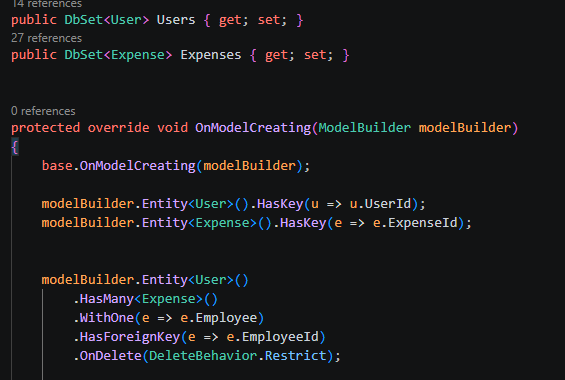
\includegraphics[width=0.6\textwidth]{Images/Implementation/AppDbContext.png}
    \caption[Code snippet from ApplicationDbContext.cs]
    {Entity Framework Core configuration in \texttt{ApplicationDbContext.cs}. [Own creation]}
    \label{fig:app-db-context}
\end{figure}

Every time the domain model changes (e.g., adding a new property to the \texttt{Expense} entity), a new database migration is created using the following .NET CLI command (included in the .NET SDK):

\begin{verbatim}
> dotnet ef migrations add <MigrationName>
\end{verbatim}

The generated migration file contains the necessary SQL scripts to update the database schema without losing existing data or causing data inconsistency. The migration is applied using the following command:

\begin{verbatim}
> dotnet ef database update
\end{verbatim}

By executing these two commands, the database stays in sync with the application's domain models.
